% !TEX root = main.tex
\chapter{Guidance Results}
\label{results}


% \begin{figure}[!htb] 
%   \centering
%   \includegraphics[width=0.5\textwidth]{alg.PNG}
%   \caption{Diagram depicting how the successive convexification loop works. If the tolerance requirements are not met, another iteration is done again to make sure it is producing dynamically feasible sets.}
%   \label{fig:succ}
%  \end{figure}

\section{Discussion}
The successive convexification routine is a very valuable tool in that it can quickly find dynamically feasible trajectories for a wide set of vehicle constraints and parameters. It could be used as an offline tool, or a receding horizon feed-forward guidance strategy where the temporal resolution increases as the terminal state constraint gets closer. It should be stated that trajectory computation employs non-dimensionalized factors for numerical stability. Tables like \ref{table:tableplanar} have been included for each of the problem statements given where all real-world values can be calculated using factors $U_L$, $U_T$ and $U_M$.


\section{Planar Problem Solutions}
Let us first study a case where the vehicle has a velocity in-plane with the terminal condition, allowing one dimension of motion to be neglected. This is the nominal scenario where a vehicle is coming in for landing and has pre-conditioned its state to do so. This is apparent in the landing of first stages, where the out-of-plane motion is canceled as much as possible and an in-plane maneuver is performed to adjust the vehicle to meet the landing pad. Figure \ref{fig:planar} shows the SCvx guidance solution to a problem with a set of initial conditions in-plane with the landing point; the vehicle has a position of 600 meters North and 500 meters east with eastward velocity of -120m/s. The incoming velocity is higher than nominal, and so the optimal control solution is to maximize the divert capability such that the lateral velocity is arrested while the attitude is upright at the final time.

\begin{table}[ht]
\caption{Parameters Used For Planar Problem}
\centering 
\begin{tabular}{c c c} 
\hline\hline
Param & Units & Value \\ [0.5ex] 
\hline 
$^\mathcal{N}\mathbf{g}$    & $U_L/U_T^2$   & $-0.108\hat{\mathbf{n}}_1$  \\ 
$\alpha_{\dot{m}}$        & -       & 0.0738  \\
$m_{wet}$             & $U_M$     & 1  \\
$m_{dry}$             & $U_M$     & 0.277  \\
$^\mathcal{N}r_{0}$       & $U_L$     & $(0.76,0.64,0)$  \\
$^\mathcal{N}v_{0}$       & $U_L/U_T$   & $(0,-0.48,0)$  \\
$\sigma_{\mathcal{B/N}_0}$    & -     & $(0,0,0.32)$  \\
$\omega_{\mathcal{B/N}_0}$    & $rad/U_T$   & $(0,0,0)$ \\[1ex] 
\hline
\end{tabular}
\begin{tabular}{c c c} 
\hline\hline
Param & Units & Value \\ [0.5ex] 
\hline 
$\gamma_{gs}$           & $deg$     & $45$  \\ 
$\delta_{max}$          & $deg$     & $10$  \\
$F_{max}$             & $U_F$     & $0.164$ \\
$F_{min}$             & $U_F$     & $0.024$  \\
$\psi_{max}$          & $deg$     & $85$  \\
$\omega_{max}$          & $deg/U_T$   & $43.84$  \\
$U_M$               & kg      & $408.233$  \\
$U_L$             & m       & $781.02$ \\
$U_T$             & s       & $3.132$ \\[1ex] 
\hline
\end{tabular}
\label{table:tableplanar}
\end{table}


\begin{figure}[!htbp] 
  \centering
  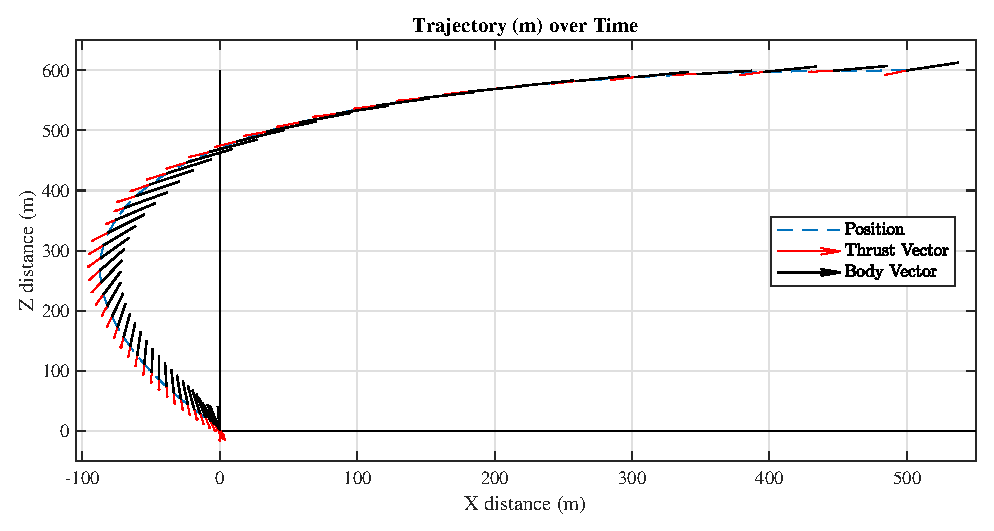
\includegraphics[width=\textwidth]{figs/planar_traj.eps}
  \caption{Planar Guidance Problem: Vehicle Descends In-line with Target}
  \label{fig:planar}
 \end{figure}
% ../SCVX/code/src/controls.eps
\begin{figure}[!htbp] 
\label{planar_controls}
  \centering
  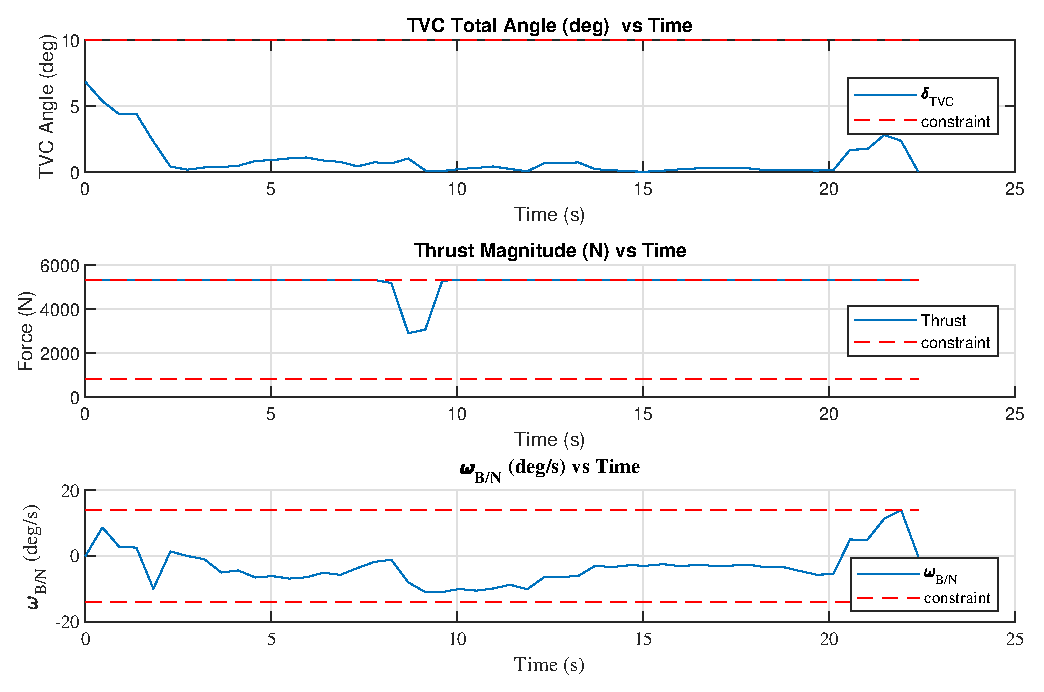
\includegraphics[width=\textwidth]{figs/planar_controls.eps}
  \caption{Planar Guidance Problem: Control and Angular Rate During Landing}
  \label{fig:planarcontrols}
 \end{figure}

\begin{figure}[!htbp] 
  \centering
  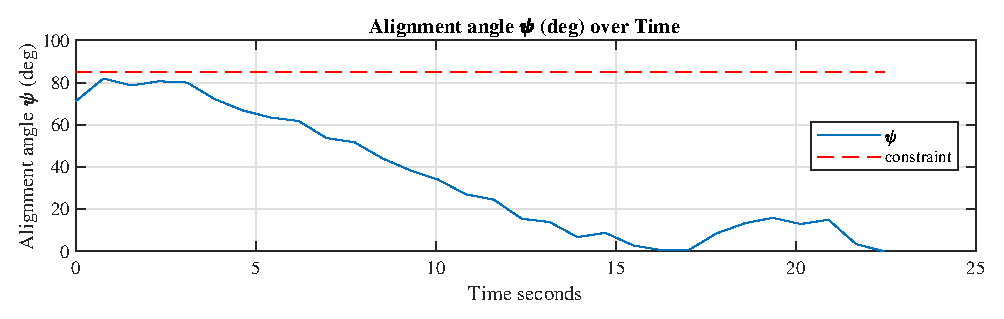
\includegraphics[width=\textwidth]{figs/planar_alignment.eps}
  \caption{Planar Guidance Problem: Total Alignment Constraint Met}
  \label{fig:nplanar_align}
 \end{figure}


 %
The control solution in figure \ref{fig:planarcontrols} shows how maximum thrust is used for nearly the entire duration where lateral thrust is used for attitude control while simultaneously lowering altitude control. The commanded TVC deflection angles stay within our proposed constraints. Our thrust magnitude and angular rate constraints are also met throughout the duration of the flight. For a fast pitch-over maneuvers like this, it is hard to find a trajectory where the vehicle angular rate maintains within reasonable boundaries; this scenario is restricted to below $14$ deg/s. All initial conditions and constraints are shown in \ref{table:tableplanar}.


The vehicle following the planar path in figure \ref{fig:planar} reached it's terminal state after $22.4$ seconds and with a final mass of $373.62$kg with a starting mass of $408.23$kg only using $11.7$\% of it's fuel. Additionally, the total alignment MRP constraint is shown to meet the requirement throughout the flight \ref{fig:nplanar_align}.


\section{Non-Planar Problem Solutions}
Now let us look at a non-planar problem where the initial condition of the vehicle is off-nominal and must make an out-of-plane maneuver to land on the target. The parameters and initial conditions are found in table \ref{table:tablenplanar}. Figure \ref{fig:nplanar} shows a vehicle coming towards the landing pad with an offset lateral position of 100m and with a velocity not pointed directly in-line with the target. All vehicle constraints are met. The vehicle uses maximum thrust almost the entire duration of the flight. The optimization provides a thrust-vectored solution which precisely arrests the attitude motion while meeting the translational requirements simultaneously. The simple MRP alignment constraint is met and shown in figure \ref{fig:nplanarcontrols}.

\begin{figure}[!htbp] 
  \centering
  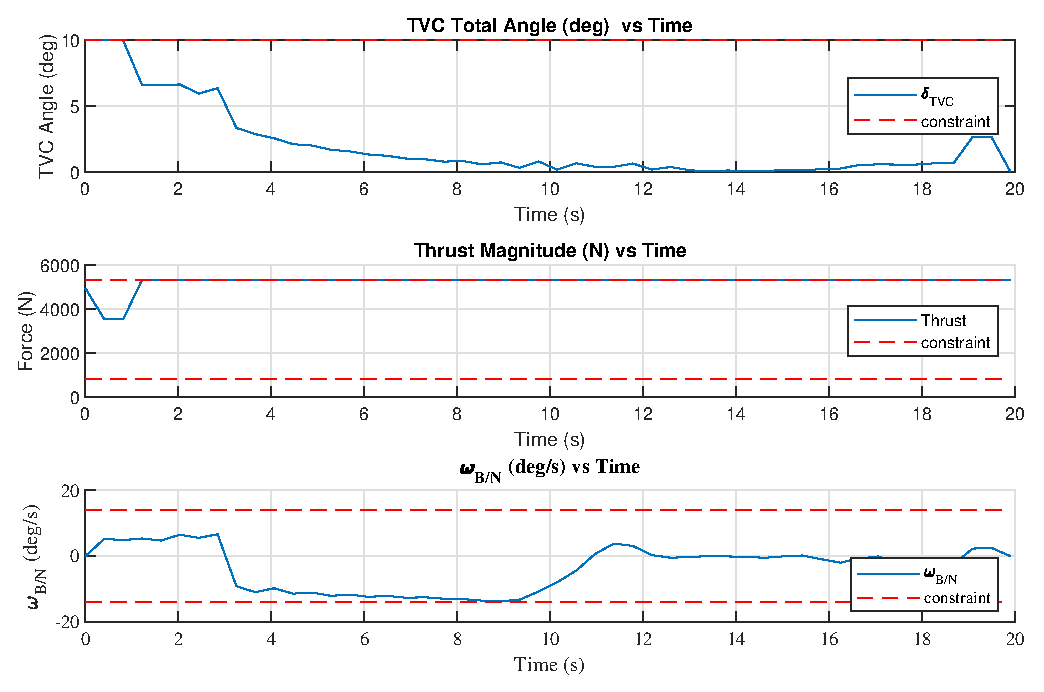
\includegraphics[width=0.65\textwidth]{figs/nonplanar_controls.eps}
  \caption{Non-Planar Guidance Problem: Controls and Angular rate of Landing Vehicle}
  \label{fig:nplanarcontrols}
 \end{figure}

\clearpage
\begin{figure}[!htbp] 
  \centering
  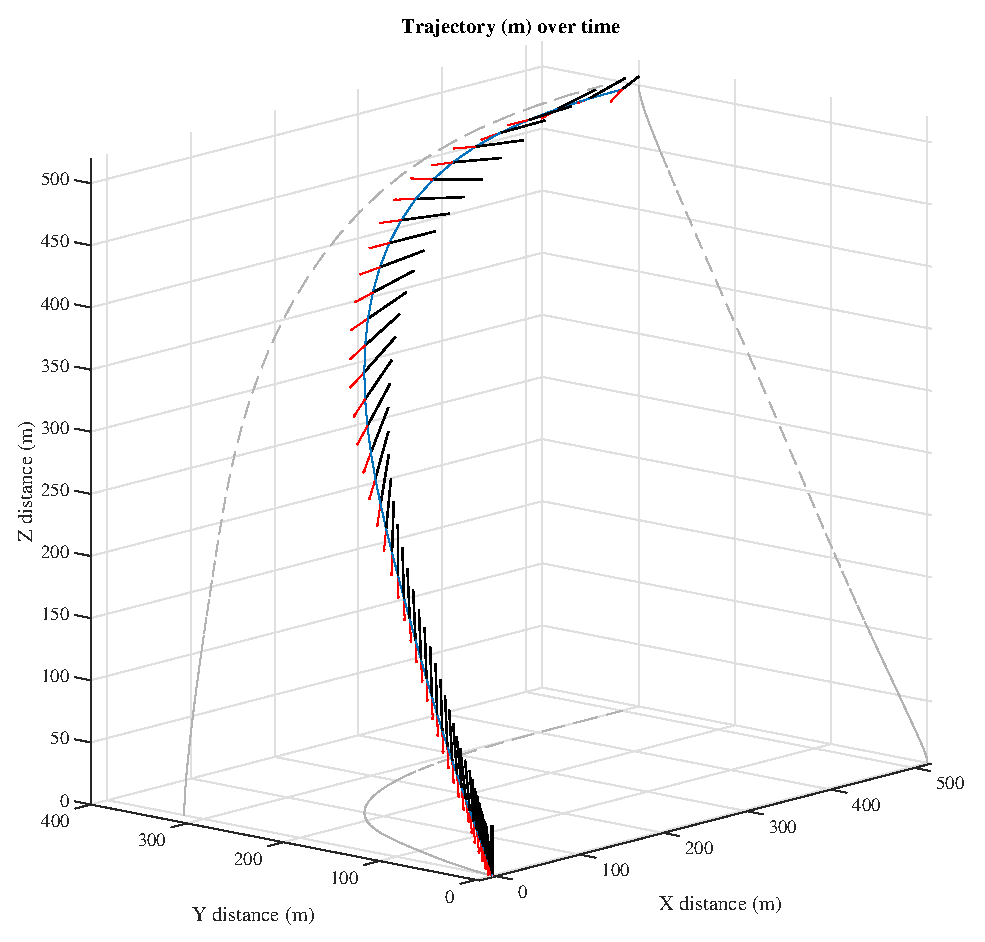
\includegraphics[width=\textwidth]{figs/nonplanar_3dtraj.eps}
  \caption{Non-Planar Guidance Problem: Vehicle Approaches Offset from Target}
  \label{fig:nplanar}
 \end{figure}

The vehicle following the non-planar path in figure \ref{fig:planar} reached its terminal state after $19.95$ seconds and with a final mass of $376.784$kg with a starting mass of $408.23$kg only using $10.6$\% of its fuel. Additionally, figure \ref{fig:nplanar_rv} shows that the terminal position and velocity constraints are met, and the vehicle reaches the landing pad with a safe terminal velocity.
\begin{figure}[ht] 
  \centering
  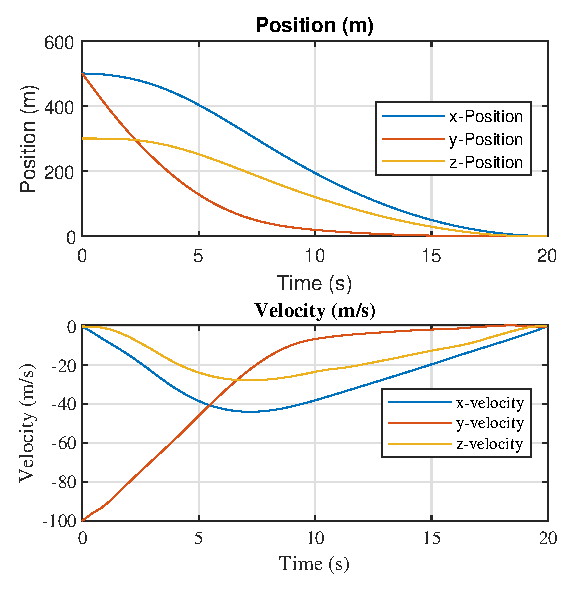
\includegraphics[width=.7\linewidth]{figs/nonplanar_rv.eps}
  \caption{Non-Planar Guidance Problem: Position and Velocity Histories}
  \label{fig:nplanar_rv}
\end{figure}
\begin{table}[ht]
  \caption{Parameters Used for Non-Planar Problem}
  \centering 
  \begin{tabular}{c c c} 
    \hline\hline
    Param & Units & Value \\ [0.5ex] 
    \hline 
    $^\mathcal{N}\mathbf{g}$ 		& $U_L/U_T^2$ 	& $\hat{\mathbf{n}}_1$  \\ 
    $\alpha_{\dot{m}}$ 				& - 			& 0.0738  \\
    $m_{wet}$ 						& $U_M$ 		& 1  \\
    $m_{dry}$ 						& $U_M$ 		& 0.277  \\
    $^\mathcal{N}r_{0}$ 			& $U_L$ 		& $(0.65,0.65,0.39)$  \\
    $^\mathcal{N}v_{0}$ 			& $U_L/U_T$	 	& $(0,-0.4,0)$  \\
    $\sigma_{\mathcal{B/N}_0}$ 		& - 			& $(0,0,0.32)$  \\
    $\omega_{\mathcal{B/N}_0}$ 		& $rad/U_T$ 	& $(0,0,0)$ \\[1ex] 
    \hline
    \end{tabular}
    \begin{tabular}{c c c} 
    \hline\hline
    Param & Units & Value \\ [0.5ex] 
    \hline 
    $\gamma_{gs}$ 					& $deg$ 		& $5$  \\ 
    $\delta_{max}$	 				& $deg$ 		& $10$  \\
    $F_{max}$ 						& $U_F$ 		& $0.166$ \\
    $F_{min}$ 						& $U_F$ 		& $0.025$  \\
    $\psi_{max}$ 					& $deg$ 		& $85$  \\
    $\omega_{max}$ 					& $deg/U_T$	 	& $43.84$  \\
    $U_M$ 							& kg 			& $408.233$  \\
    $U_L$					 		& m			 	& $768.114$ \\
    $U_T$					 		& s			 	& $3.132$ \\[1ex] 
    \hline
  \end{tabular}
  \label{table:tablenplanar}
\end{table}










% \begin{figure}[!htbp] 
%   \centering
%   \includegraphics[width=0.7\linewidth]{thrusters.png}
%   \caption{Plot of the output thrust of each of the thrusters for the non-nominal initial attitude case.}
%   \label{fig:thrusty}
%  \end{figure}